\subsection{Aufbau des Touchscreen GUI's}
	Nun also zur Software. Kern des Systems ist eine Abstraktion des Touchscreens auf dem Daughterboard:
	
	\subsubsection{Die Klasse TouchScreen}\label{sec:touchscreen_class}
		\begin{wrapfigure}{r}{0.4\textwidth}
			\scalebox{0.75}{
				\begin{tikzpicture}
					\begin{class}[text width=7.5cm]{TouchScreen}{0, 0}
	\attribute{- x, y: WORD}
	\attribute{- touchCount: WORD}
	\attribute{- width, height: WORD}
	\attribute{- i2cTouch: cHwI2Cmaster::Device\&}
	\attribute{- interruptPort: cHwPort\_N::PortId}
	\attribute{+ interruptPin: BYTE}
	\attribute{+ rootContainer: Container*}
	\attribute{+ \emph{static} INSTANCE: TouchScreen*}
	
	\operation{+ refresh(): void}
	\operation{+ setInterruptMode(mode: bool): void}
	\operation{+ interruptHandler(): void}
	\operation{+ setRootContainer(c: Container*): void}
	\operation{+ getRootContainer(): Container*}
\end{class}
				\end{tikzpicture}
			}
		\end{wrapfigure}
		Diese Klasse bietet verschiedene Methoden, welche die Kommunikation mit dem Daughterboard umsetzen und ist als \emph{Singelton} entworfen.
		Die statische Variable \texttt{INSTANCE} speichert die (einzige) Instanz dieser Klasse, um ihren \texttt{interruptHanlder} aus \texttt{linkage "C"} aufrufen zu können.
		Um das System nicht unnötig aus zu lasten, ist die Instanz in der Lage, einen GPIO-Interrupt zu behandeln.
		Sobald eine Berührung erkannt wird, fragt \texttt{refresh()} die aktuellen Daten über den I²C-Bus vom Daughterboard ab und löst ein entsprechendes \secref{EventSystem}{Event} aus. Dieses Event wird an den \texttt{RootContainer} übergeben, welcher es an seine Komponenten weitergibt.
	
	\subsubsection{Komponenten und Container}\label{sec:components}
		\begin{wrapfigure}{r}{0.4\textwidth}
			\scalebox{0.75}{
				\begin{tikzpicture}
					\begin{abstractclass}[text width=11cm]{Component}{0, 0}
	\attribute{\# box: BoundingBox}
	
	\operation{+ Component(x: WORD, y: WORD, w: WORD, h: WORD)}
	\operation{+ getBoundingBox(): BoundingBox\&}
	\operation[0]{+ onEvent(event: DragEvent\&): void}
	\operation[0]{+ onEvent(event: TouchEvent\&): void}
	\operation[0]{+ onEvent(event: ReleaseEvent\&): void}
	\operation[0]{+ show(display: cDevDispalyGraphic\&): void}
\end{abstractclass}
				\end{tikzpicture}
			}
			\label{uml-component}
			%\caption{Component UML}
		\end{wrapfigure}
		Alle Komponenten haben die gemeinsame Oberklasse \texttt{Component}, welche drei Aspekte der Komponenten modelliert. Erstens: die \texttt{BoundingBox}, ein achsparalleles Rechteck, welches die Komponente vollständig enthält.
		Eine Komponente erhält Touchscreen-Events nur, wenn diese in ihrer \texttt{BoundingBox} liegen.
		Zweitens: drei Methoden, welche Touchscreen-Events annehmen und verarbeiten.
		Drittens: eine Methode, welche die Komponente auf ein Display zeichnen kann.
		
		Einzelne Komponenten können eigene Events auslösen (\texttt{ActionEvents}).
		Diese sind aber komponentenspezifisch und deswegen nicht in der Klasse \texttt{Component} implementiert.
		
		\medskip
		\begin{wrapfigure}{r}{0.4\textwidth}
			\scalebox{0.75}{
				\begin{tikzpicture}
					\begin{abstractclass}{Component}{0, 0}
					\end{abstractclass}
				
					\begin{class}[text width=11cm]{Container}{0, -2.5}
	\inherit{Component}
	
	\attribute{- compontents: list<Component*>}
	
	\operation{+ addComponent(comp: Component*): void}
	\operation{+ removeComponent(comp: Component*): void}
\end{class}
				\end{tikzpicture}
			}
			\label{uml-container}
		%\caption{Container UML}
		\end{wrapfigure}
		Ein \texttt{Container} dient nur dazu, mehrere Komponenten in einer Gruppe zusammenzufassen.
		Bestände die Möglichkeit, eine Komponente zu \emph{deaktivieren}, wäre es Aufgabe dieser Klasse diese Operation an ihre Komponenten weiterzugeben.
		Beispielsweise könnte eine Gruppe von \texttt{RadioButtons} -- in einem Container zusammengefasst -- durch nur einen Aufruf deaktiviert werden.
		Dieses Feature ist aber nicht implementiert, demnach ist der \texttt{Container} nur eine logische Einheit.
		
		\medskip
		\begin{wrapfigure}{r}{0.4\textwidth}
			\scalebox{0.75}{
				\begin{tikzpicture}
					\begin{abstractclass}{Component}{-3, 0}
					\end{abstractclass}
				
					\node[right=of Component] (image) {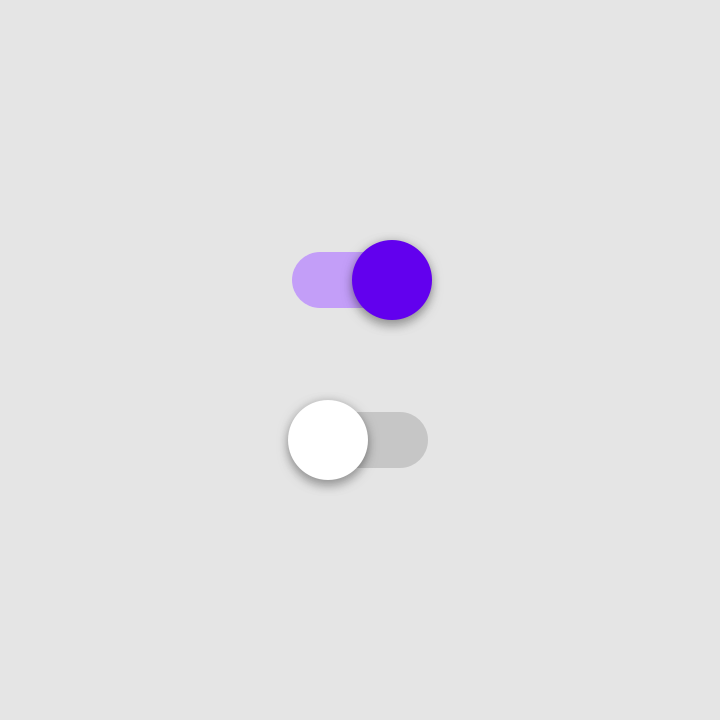
\includegraphics[height=2cm]{../Images/Switch.png}~\cite{material-components}};
					
					\begin{class}[text width=11cm]{ToggleSwitch}{0, -2.5}
	\inherit{Component}
	
	\attribute{- state: bool}
	\attribute{- listeners: list<function<void(ToggleSwitchEvent\&)>\relax>}
	
	\operation{+ getState(): bool}
	\operation{+ addEventListener(listener: function<void(ToggleSwitchEvent\&)>): void}
\end{class}
				\end{tikzpicture}
			}
			\label{uml-toggleswitch}
			%\caption{ToggleSwitch UML}
		\end{wrapfigure}
		Ein \texttt{ToggleSwitch} dient zum Setzen einer Ein/Aus-Einstellung.
		Dementsprechend speichert die Klasse \texttt{ToggleSwitch} den aktuellen Zustand des Schalters in einem \texttt{bool}.
		Erhält ein \texttt{ToggleSwitch} ein \texttt{TouchEvent} wechselt er den Zustand.
		Außerdem erzeugt er ein \texttt{ToggleSwitchEvent} (eine Subklasse von \texttt{ActionEvent}).
		Dieses wird dann an alle über die Methode \texttt{addEventListener} hinzugefügten Funktionen übergeben.
		Ändert sich der Zustand, dann enthält das korrespondierende \texttt{ActionEvent} den neuen Zustand und wird an alle registrierten \texttt{Listener} übergeben.
		
		\medskip
		\begin{wrapfigure}{r}{0.4\textwidth}
			\scalebox{0.75}{
				\begin{tikzpicture}
					\begin{abstractclass}{Component}{-3, 0}
					\end{abstractclass}
					
					\node[right=of Component] (image) {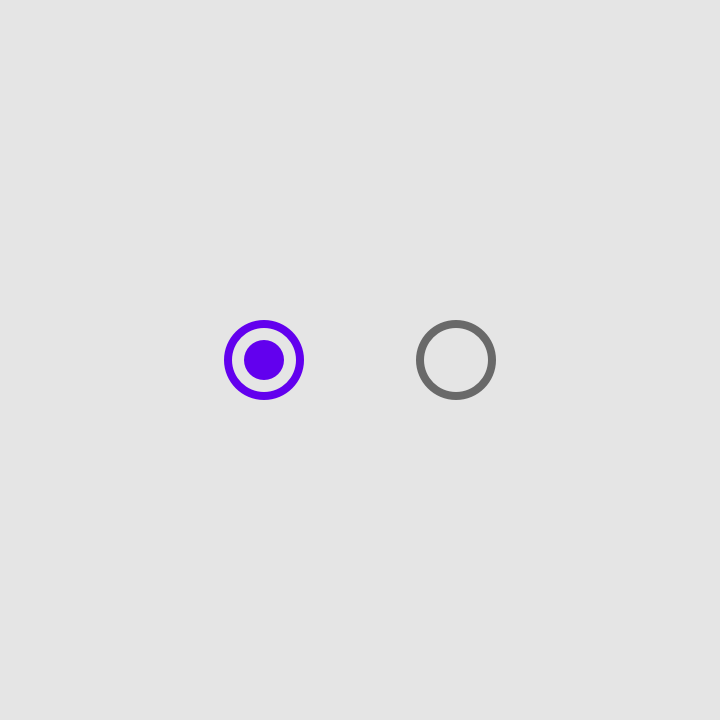
\includegraphics[height=2cm]{../Images/RadioButton.png}};
					
					\begin{class}[text width=11cm]{RadioButton}{0, -2.5}
	\inherit{Component}
	
	\attribute{- state: bool}
	\attribute{- deselectable: bool}
	\attribute{- listeners: list<function<void(RadioButtonEvent\&)>\relax>}
	
	\operation{+ getState(): bool}
	\operation{+ addEventListener(listener: function<void(RadioButtonEvent\&)>): void}
\end{class}
				\end{tikzpicture}
			}
			\label{uml-radiobutton}
			%\caption{RadioButton UML}
		\end{wrapfigure}
		Wie ein \texttt{ToggleSwitch} dient ein \texttt{RadioButton} zum Setzen einer Ein/Aus-Einstellung.
		Im Gegensatz zu einem \texttt{ToggleSwitch} kommuniziert ein \texttt{RadioButton} sich gegenseitig ausschließende Optionen.
		Die beiden Klassen ähneln sich daher stark. Der einzige Unterschied liegt darin, dass es möglich ist, das Abwählen eines
		\texttt{RadioButtons} im Konstruktor zu deaktivieren. Ein \texttt{RadioButton} kann dann nur abgewählt werden,
		indem ein anderer Button der selben Gruppe (also eine andere Option) ausgewählt wird.
		
		\medskip
		\begin{wrapfigure}{r}{0.4\textwidth}
			\scalebox{0.75}{
				\begin{tikzpicture}
					\begin{abstractclass}[text width=3cm]{Component}{-4, 0}
					\end{abstractclass}
					
					\node[right=of Component] (image) {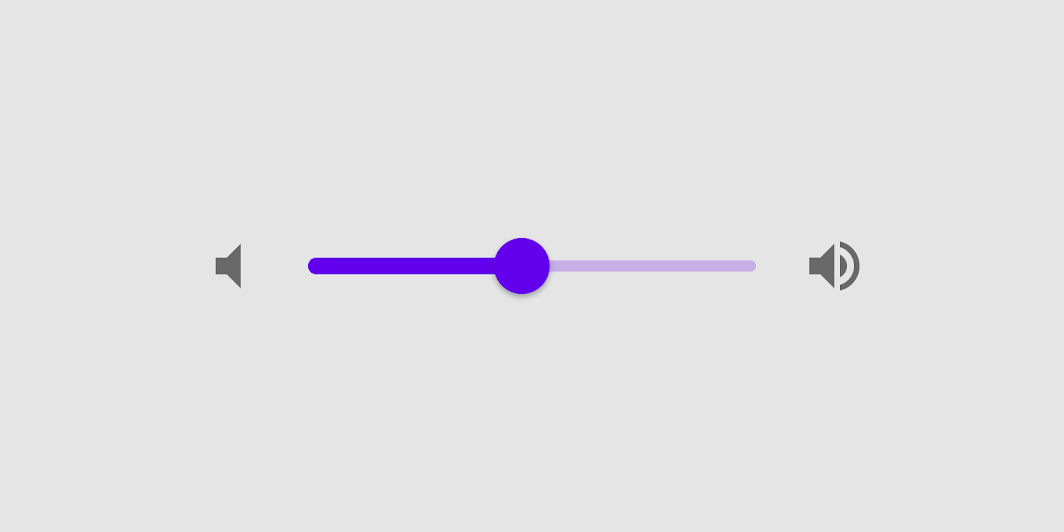
\includegraphics[height=2cm]{../Images/Slider.png}};
					
					\begin{class}[text width=11cm]{Slider}{0, -2.5}
	\inherit{Component}
	
	\attribute{- position: double}
	\attribute{- listeners: list<function<void(SliderEvent\&)>\relax>}
	
	\operation{- setPosition(x: WORD): void}
	\operation{+ getPosition(): double}
	\operation{+ addEventListener(listener: function<void(SliderEvent\&)>): void}
\end{class}
				\end{tikzpicture}
			}
			\label{uml-slider}
			%\caption{Slider UML}
		\end{wrapfigure}
		Ein \texttt{Slider} ermöglicht das Auswählen eines Wertes aus einem stetigen Bereich.
		
	\subsubsection{Event System}\label{sec:EventSystem}